\chapter{2019}
\section*{一、选择题(本大题共 10 小题,每小题 2 分,共 20 分)}

1. 对于双向循环链表, 每个结点有两个指针域 next 和 prior, 分别指向前驱和后继。在 \(\mathrm{p}\) 指针所指向的结点之后插入 \(\mathrm{s}\) 指针所指结点的操作应为(   )。

A. p->next = s; s->prior = p; p->next->prior = s; s->next = p->next;

B. p->next = s; p->next->prior = s; s->prior = p; s->next;

C. s->prior = p; s->next = p->next; p->next = s; p->next->prior = s;

D. s->prior = p; s->next = p->next; p->next->prior = s; p->next = s;

2. 由 abc,3 个结点可以构造出多少种不同的二叉树? (   )

A. 2 B. 3 C. 4 D. 5

3. 设有数组 \(\mathrm{A}\left\lbrack  {\mathrm{i},\mathrm{j}}\right\rbrack\) ,数组的每个元素长度为 3 字节, \(\mathrm{i}\) 的值为1到 \(8,\mathrm{j}\) 的值为 1 到 10 , 数组从内存首地址 BA 开始顺序存放, 当用以列为主存放时, 元素 A[5, 8]的存储首地址为(   )。

A. BA+141 B. BA+180 C. BA+222 D. BA+225

4. 一个栈的输入序列为 123 ,则下列序列中不可能是栈的输出序列的是(   )。

A.231 B. 3 2 1

C. 3 1 2 D. 1 2 3

5. 下述编码中哪一个不是前缀码(   )。

A.(00,01,10,11) B.(0,1,00,11)

C.(0,10,110,111) D.(1,01,000,001)

6. 当一棵有 n 个结点的二叉树按层次从上到下,同层次从左到右将数据存放在一维数组 A[l..n]中时,数组中第 i 个结点的左孩子为(   )。

A. \(\mathrm{A}\left\lbrack  {2\mathrm{i}}\right\rbrack  \left( {2\mathrm{i} =  < \mathrm{n}}\right)\) B. \(\mathrm{A}\left\lbrack  {2\mathrm{i} + 1}\right\rbrack  \left( {2\mathrm{i} + 1 =  < \mathrm{n}}\right)\) C. \(A\left\lbrack  {i/2}\right\rbrack\) D. 无法确定

7. 假设一个有 \(\mathrm{n}\) 个顶点和 \(\mathrm{e}\) 条弧的有向图用邻接表表示,则删除与某个顶点 vi 相关的所有弧的时间复杂度是(   )。

A. O(n) B. \(\mathrm{O}\left( \mathrm{e}\right)\) C. \(\mathrm{O}\left( {\mathrm{n} + \mathrm{e}}\right)\) D. \(\mathrm{O}\left( {{\mathrm{n}}^{ * }\mathrm{e}}\right)\)

8. 串的长度是指(   )。

A. 串中所含不同字母的个数 B. 串中所含字符的个数

C. 串中所含不同字符的个数 D. 串中所含非空格字符的个数

9. 循环队列存储在数组 \(\mathrm{A}\left\lbrack  {0..\mathrm{m}}\right\rbrack\) 中,则入队时的操作为(   )。

A. rear=rear+1 B. rear=(rear+1) mod (m-1)

C. rear=(rear+1) mod m D. rear=(rear+1)mod(m+1)

10. 关键路径是事件结点网络中(   )。

A. 从源点到汇点的最长路径 B. 从源点到汇点的最短路径

C. 最长回路 D. 最短回路

\section*{二、填空题(本大题共 15 小题,每空 2 分,共 40 分)}

1. 中缀算式 (3+4X) -2Y/3 对应的后缀算式为\_\_\_\_\_。

2. 在完全二叉树中,编号为 \(\mathrm{i}\) 和 \(\mathrm{j}\) 的两个结点处于同一层的条件是\_\_\_\_\_。

3. 构造 n 个结点的强连通图,至少有\_\_\_\_\_条弧。

4. 设有一个空栈,栈顶指针为 \({1000}\mathrm{H}\) (十六进制),现有输入序列为 \(\mathrm{a},\mathrm{b},\mathrm{c},\mathrm{d}\) ,
e. 经过 PUSH, PUSH, POP, PUSH, POP, PUSH, PUSH 之后,输出序列是\_\_\_\_\_, 而栈顶指针值是\_\_\_\_\_ \(\mathrm{H}\) 。设栈为顺序栈,每个元素占 4 个字节。

5. 若串 S1=‘ABCDEFG’, S2=‘9898’, S3=‘\#\#\#’, S4=‘012345’, 执行 concat(replace(S1, substr(S1, length(S2), length(S3)), S3), substr(S4, index(S2,‘8’), lengt h(S2))),其结果为\_\_\_\_\_。

6. 若一组记录的排序码为(46,79,56,38,40,84),则利用堆排序的方法建立的初始堆为\_\_\_\_\_。

7. 在有序表 (12,24,36,48,60,72,84) 中二分查找关键字 72 时所需进行的关键字比较次数为\_\_\_\_\_。

8. 有向图的边集为 \(\{  < \mathrm{a},\mathrm{c} > , < \mathrm{a},\mathrm{e} > , < \mathrm{e},\mathrm{b} > , < \mathrm{e},\mathrm{d} > , < \mathrm{b},\mathrm{d} > , < \mathrm{d},\mathrm{c} > , < \mathrm{c},\mathrm{f} > \}\) ,该图的一个拓扑排序为:\_\_\_\_\_。

注:所有答案必须写在答题纸上, 试卷上作答无效 !

9. 当输入序列局部有序或元素个数较小时, 在快速排序、选择排序、插入排序、 归并排序、堆排序中,最佳的排序方法是\_\_\_\_\_。

10. 假设两个队列共享一个循环向量空间 (参见右图), 其类型 Queue2 定义如下:

\begin{center}
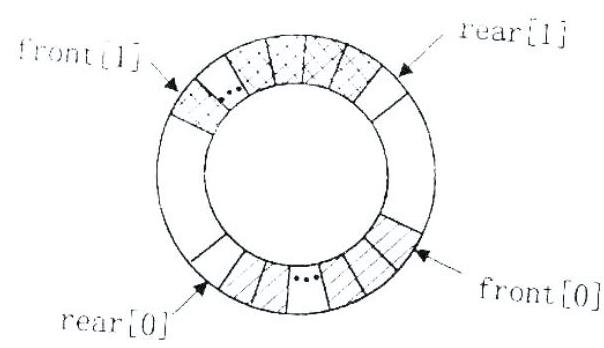
\includegraphics[width=0.5\textwidth]{images/2019/blank_10.jpg}
\end{center}
\hspace*{3em} 

\begin{lstlisting}[language=C, basicstyle=\ttfamily]
    typedef struct {
        DateType data[MaxSize];
        int front[2],rear[2];
    } Queue2;
\end{lstlisting}

对于i=0或l,front[i]的和rear[i]的分别为第i个队列的头指针和尾指针。请对以下算法填空，实现第i个队列的入队操作。

\begin{lstlisting}[language=C, basicstyle=\ttfamily]
int EnQueue(Queue2 *Q,int i,DateType x)
{    //若第i个队列不满，则元素x入队列，并返回1：否则返回0
    if(i<0 || i>1)
        return 0;
    if(Q->rear[i]==Q->front[          ]) return 0;
    Q->data[          ]=x;
    Q->rear[i]=[          ];
    return1;
}
\end{lstlisting}


11. 高度为 8 的平衡二叉树的结点数至少有\_\_\_\_\_个。

12. 文件由\_\_\_\_\_组成；记录由\_\_\_\_\_组成。

13. 对于一个具有 \(\mathrm{n}\) 个结点的单链表,在已知的结点*p 后插入一个新结点的时间复杂度为\_\_\_\_\_,在给定值为 \(\mathrm{x}\) 的结点后插入一个新结点的时间复杂度为\_\_\_\_\_。

14. 在 n 个记录的有序顺序表中进行折半查找,最大比较次数是\_\_\_\_\_。 

15. 求从某源点到其余各顶点的 Dijkstra 算法在图的顶点数为 10 ,用邻接矩阵表示图时计算时间约为 10ms,则在图的顶点数为 40,计算时间约为\_\_\_\_\_ms。

\section*{三、问答题(本大题共 6 小题,每小题 10 分,共 60 分)}

1. 一个线性表为 B=(12,23,45,57,20,03,78,31,15,36),设散列表为 \(\mathrm{{HT}}\left\lbrack  {0.12}\right\rbrack\) ,散列函数为 \(\mathrm{H}\left( \mathrm{{key}}\right)  = \mathrm{{key}}\% {13}\) 并用线性探查法解决冲突,请画出散列表, 并计算等概率情况下查找成功的平均查找长度。
\vspace{10em}

2. 已知二叉树的存储结构为二叉链表,阅读下面算法。

\begin{lstlisting}[language=C, basicstyle=\ttfamily]
typedef struct node {
    DateType data;
    struct node *next;
} ListNode;
typedef ListNode *LinkList;
LinkList Leafhead = NULL;
void Inorder (BinTree T)
{
    LinkList s;
    if(T)
    {
        Inorder(T->lchild);
        if ((!T->lchild)&&(!T->rchild))
            {
                s=(ListNode*)malloc(sizeof(ListNode));
                s->data = T->data;
                s->next = Leafhead;
                Leafhead=s;
            }
        Inorder(T->rchild);
    }
}
\end{lstlisting}

对于如下所示的二叉树
\begin{center}
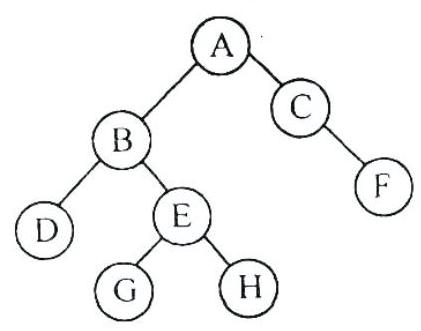
\includegraphics[width=0.4\textwidth]{images/2019/ask_2.jpg}
\end{center}
\hspace*{3em} 

(1)画出执行上述算法后所建立的结构

(2)说明该算法的功能
\vspace{10em}

\newpage
3. 假设以 I 和 O 分别表示入栈和出栈操作。栈的初态和终态均为空,入栈和出栈的操作序列可表示为仅由 \(\mathrm{I}\) 和 \(\mathrm{O}\) 组成的序列,称可以操作的序列为合法序列, 否则称为非法序列。

(1)下面所示的序列中哪些是合法的?

A. IOIIOIOO B. IOOIOIIO C. IIIOIOIO D. IIIOOIOO

(2)通过对(1)的分析,写出一个算法,判定所给的操作序列是否合法。(假定被判定的操作序列已存入一维数组 char A[ ]中, 若操作序列合法, 返回 true, 否则返回 false)。
\vspace{10em}

4. 已知一个连通图如下图所示, 试给出图的邻接矩阵和邻接表存储示意图,若从顶点 \(\mathrm{v}1\) 出发对该图进行遍历, 分别给出一个按深度优先遍历和广度优先遍历的顶点序列.

\begin{center}
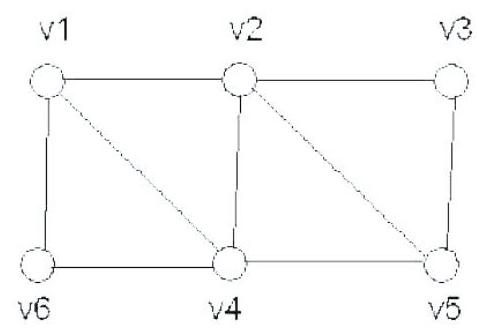
\includegraphics[width=0.4\textwidth]{images/2019/ask_4.jpg}
\end{center}
\hspace*{3em} 

(1)图的邻接矩阵

(2)邻接表存储示意图

(3)从 v1 开始的深度优先遍历的顶点序列

(4)分析在深度遍历过程中,分别使用邻接矩阵和邻接表存储的算法复杂度

( 5 )讨论在图遍历问题中,这两种存储方式的优劣 
\vspace{10em}

\newpage
5. 一棵二叉树的先序序列为 ABCDGEF, 中序序列为 CBDGAFE。 

(1)请画出该二叉树

(2)将二叉树转换为相应的森林
\vspace{10em}

6. 请阅读下列算法,回答问题
\begin{lstlisting}[language=C, basicstyle=\ttfamily]
sort(r,n)
{
    for (i=2;i<=n;i++)
    { 
        x=r[i]; r[0]=x; j=i-1;
        while(x<r[j])
            {
                r[j+1]=r[j];
                j=j-1;
            }
        r[j+1]=x;
    }
}
\end{lstlisting}

(1)这是什么类型的排序算法, 该排序算法稳定吗?

(2)设置 \(\mathrm{r}\left( 0\right)\) 的作用是什么？

(3)若将 while 语句中判断条件改为 \(x <  = r\left( j\right)\) ,该算法将会有什么变化？

(4)若将 while 语句中判断条件改为 \(x <  = r\left( j\right)\) ,该算法是否还能正确工作?
\vspace{10em}

\section*{四、程序设计题 (本大题共 2 小题, 每小题 15 分, 共 30 分)}

1. 设有大小不等的 \(\mathrm{n}\) 个数据组,其数据总量为 \(\mathrm{m}\) ,顺序存放在空间 \(\boxtimes  \mathrm{D}\) 内,每个数据占一个存储单元,数据组的首地址由数组 \(\mathrm{S}\) 给出,(如下图所示),试编写将新数据 \(\mathrm{x}\) 插入到第 \(\mathrm{i}\) 个数据组的末尾且属于第 \(\mathrm{i}\) 个数据组的算法,插入后,空间区 \(\mathrm{D}\) 和数组 \(\mathrm{S}\) 的相互关系仍保持正确。

\begin{center}
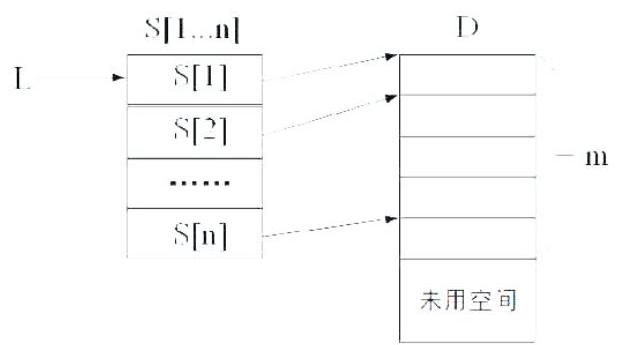
\includegraphics[width=0.5\textwidth]{images/2019/program_1.jpg}
\end{center}
\hspace*{3em} 
\vspace{15em}

2. 快速排序算法中, 如何选取一个界值 (又称为轴元素), 影响着快速排序的效率, 而且界值也并不一定是被排序序列中的一个元素。例如, 我们可以用被排序序列中所有元素的平均值作为界值。用 \(\mathrm{C}\) 语言编写算法实现以平均值为界值的快速排序方法(注:待排序数据存储在数组 \(\mathrm{R}\left\lbrack  \right\rbrack\) 中,数组最小下标为 \(\mathrm{S}\) ,数组最大下标为 T)。